\chapter{Modelar Diagrama de Caso de Uso}

Essa atividade do processo tem como objetivo listar os casos de uso, definir as relações dos atores com seus respectivos casos de uso, e quais as generalizações de usuários que foram decididas. Esse diagrama tem como objetivo mostrar o sistema em alto nível, no ponto de vista dos usuários.

O diagrama de caso de uso que modelamos para o software completo (não desenvolvido nessa disciplina) é o da figura \ref{fig:diagrama-caso-uso}.

\begin{figure}[H]
  \center
  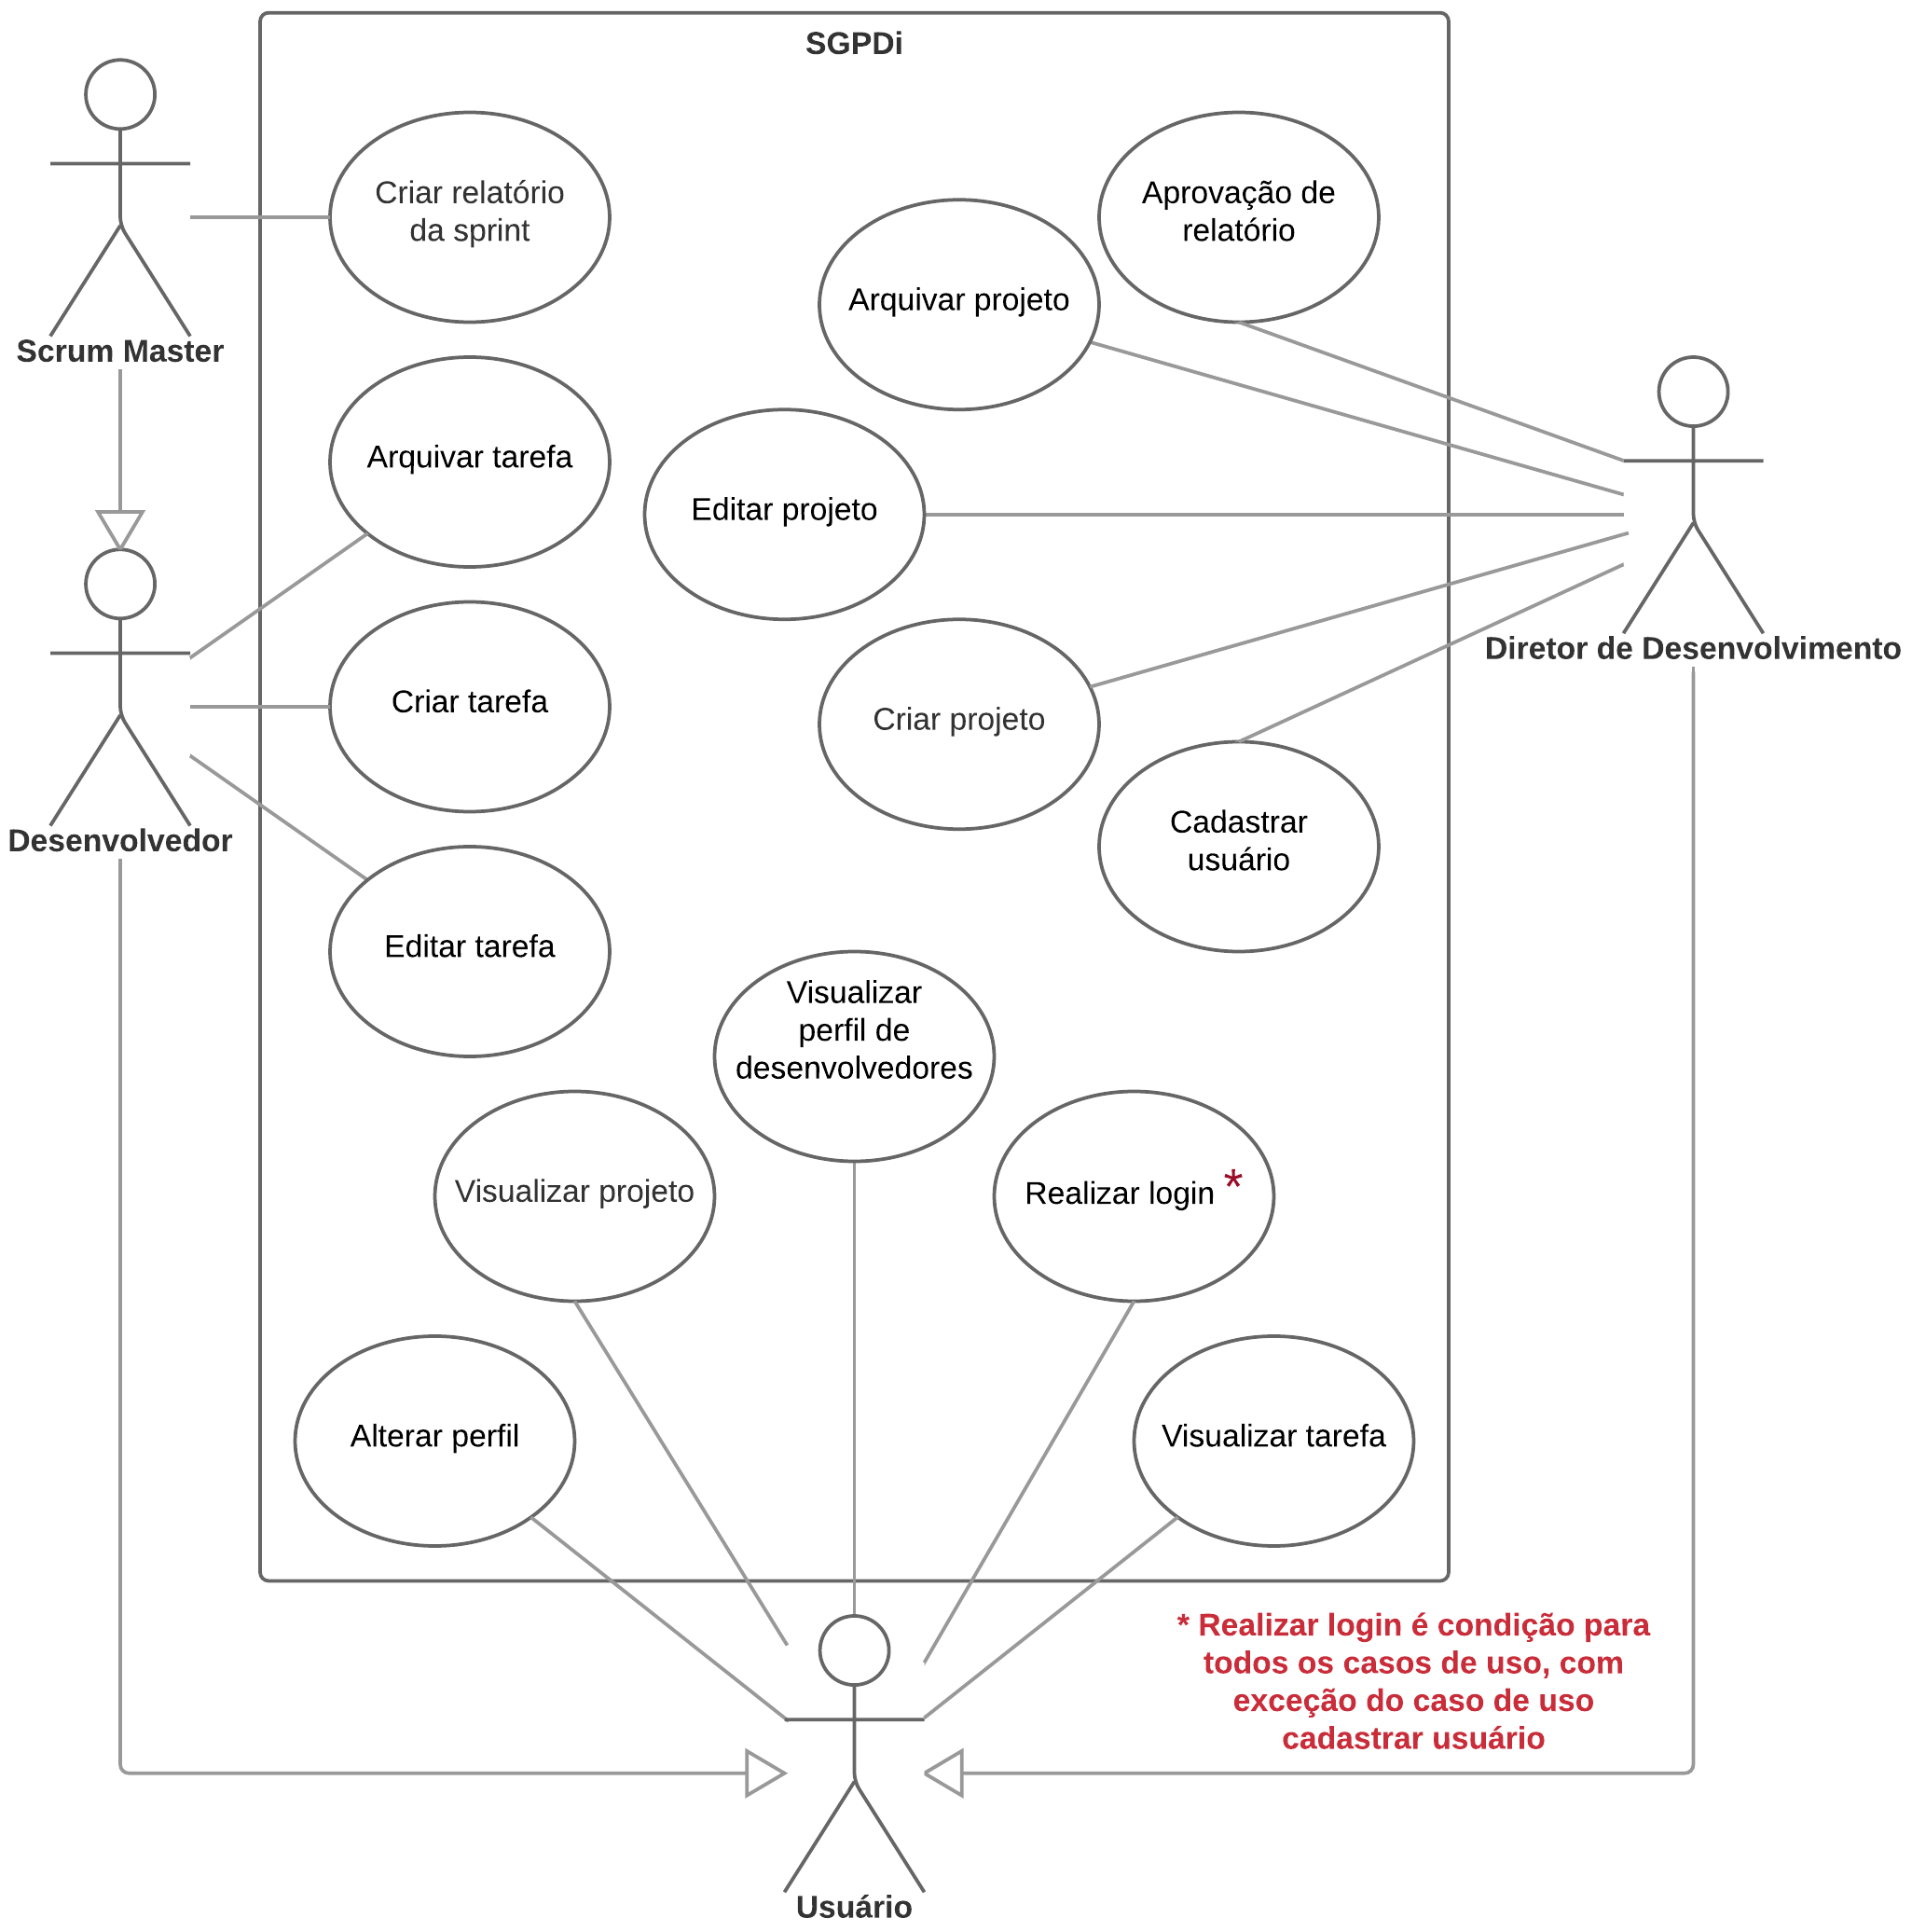
\includegraphics[width=0.7\textwidth]{figuras/diagrama-caso-uso.png}
  \caption{Diagrama de Caso de Uso}
  \label{fig:diagrama-caso-uso}
\end{figure}
